\documentclass[conference]{IEEEtran}
\IEEEoverridecommandlockouts
% The preceding line is only needed to identify funding in the first footnote. If that is unneeded, please comment it out.
\usepackage{cite}
\usepackage{amsmath,amssymb,amsfonts}
\usepackage{algorithmic}
\usepackage{graphicx}
\usepackage{textcomp}
\usepackage{xcolor}
\usepackage{listings}
\lstset{
    basicstyle=\ttfamily\footnotesize, 
    breaklines=true,                   
    frame=single,                      
    columns=fullflexible
}
\def\BibTeX{{\rm B\kern-.05em{\sc i\kern-.025em b}\kern-.08em
    T\kern-.1667em\lower.7ex\hbox{E}\kern-.125emX}}
\begin{document}

\title{Proyecto 1\\
}

\author{
    \IEEEauthorblockN{Edgar André Araya Vargas}
    \IEEEauthorblockA{
        \textit{Ingeniería en Computación} \\
        \textit{Instituto Tecnológico de Costa Rica}\\
        Cartago, Costa Rica \\
        andrearaya1234@estudiantec.cr
    }
\and
\IEEEauthorblockN{2\textsuperscript{nd} Given Name Surname}
\IEEEauthorblockA{\textit{dept. name of organization (of Aff.)} \\
\textit{name of organization (of Aff.)}\\
City, Country \\
email address or ORCID}
}

\maketitle

\begin{abstract}

\end{abstract}

\begin{IEEEkeywords}

\end{IEEEkeywords}

\section{Introducción}

El campo del Machine Learning ha experimentado un crecimiento exponencial en los últimos años, ofreciendo soluciones innovadoras a problemas complejos en diversas áreas. Este proyecto se centra en la aplicación de técnicas de clasificación de datos a dos conjuntos de datos distintos, con el objetivo de explorar y comparar diferentes herramientas de Machine Learning, contribuyendo así al desarrollo del conocimiento a través de la investigación aplicada.

El primer conjunto de datos, proporcionado por el Instituto Nacional de Diabetes y Enfermedades Digestivas y Renales, se enfoca en la predicción diagnóstica de diabetes. Este dataset incluye diversas mediciones médicas y demográficas de pacientes, como el número de embarazos, nivel de glucosa, presión arterial, grosor del pliegue cutáneo, insulina, índice de masa corporal (BMI), función de pedigrí de diabetes y edad. El objetivo es desarrollar un modelo capaz de predecir con precisión si un paciente tiene diabetes basándose en estas variables.

El segundo conjunto de datos, seleccionado por nuestro equipo, se relaciona con la rotación de empleados (attrition) de IBM. Este dataset contiene una amplia gama de variables relacionadas con los empleados, incluyendo edad, tasa de salario, departamento, distancia desde el hogar, educación, satisfacción laboral, ingresos mensuales y años en la empresa, entre otros. El análisis de este conjunto de datos busca identificar factores que puedan influir en la retención de empleados, un tema de gran relevancia en la gestión de recursos humanos y la estrategia empresarial.

La elección de estos dos conjuntos de datos permite abordar problemas de clasificación en contextos muy diferentes: uno en el ámbito de la salud y otro en el ámbito empresarial. Esta diversidad enriquece el proyecto, permitiendo explorar la versatilidad y eficacia de las técnicas de Machine Learning en escenarios distintos.

\section{Metodología}

Para abordar los objetivos del proyecto, se ha diseñado una metodología estructurada que abarca desde la exploración inicial de los datos hasta la evaluación comparativa de los modelos de clasificación. A continuación, se detallan los pasos principales:

\subsection{Exploración y Preprocesamiento de Datos}

Para ambos conjuntos de datos (Diabetes e IBM Attrition), se realizará un análisis exploratorio exhaustivo:

\begin{enumerate}
    \item \textbf{Análisis estadístico básico:} Se examinarán las distribuciones de las variables, medidas de tendencia central y dispersión.
    \item \textbf{Manejo de valores faltantes:} Se identificarán y tratarán los valores faltantes mediante reemplazo por la mediana.
    \item \textbf{Detección y tratamiento de outliers:} Se identificarán valores atípicos y se decidirá cómo manejarlos basándose en el contexto de cada variable.
    \item \textbf{Análisis de balance de clases:} Se evaluará la distribución de las clases objetivo (diabetes/no diabetes, attrition/no attrition) utilizando visualizaciones con matplotlib o seaborn.
    \item \textbf{Justificación de observaciones:} Se documentarán y justificarán todas las decisiones tomadas durante el preprocesamiento.
\end{enumerate}

\subsection{Preparación de Datos para Modelado}

\begin{enumerate}
    \item \textbf{División del conjunto de datos:}
    \begin{itemize}
        \item 70\% para entrenamiento
        \item 15\% para validación
        \item 15\% para testing
    \end{itemize}
    \item Normalización/Estandarización de características numéricas si es necesario.
    \item Codificación de variables categóricas (especialmente relevante para el conjunto de datos de IBM Attrition).
\end{enumerate}

\subsection{Desarrollo y Evaluación de Modelos}

Se implementarán dos modelos de clasificación para cada conjunto de datos:

\begin{enumerate}
    \item Regresión Logística
    \item K-Nearest Neighbors (KNN)
\end{enumerate}

Para cada modelo:
\begin{itemize}
    \item Se realizarán múltiples ejecuciones con diferentes hiperparámetros.
    \item Se utilizará el conjunto de validación para verificar la convergencia y evitar el sobreajuste.
    \item Se mantendrán constantes los conjuntos de entrenamiento y prueba para asegurar la comparabilidad entre experimentos.
\end{itemize}

\subsection{Evaluación de Modelos}

La evaluación de los modelos se realizará utilizando el conjunto de datos de prueba. Se calcularán las siguientes métricas:

\begin{itemize}
    \item Accuracy
    \item Precision
    \item Recall
    \item Matriz de confusión
\end{itemize}

Además, se realizará una comparación detallada entre los modelos de regresión logística y KNN para cada conjunto de datos, analizando sus fortalezas y debilidades en el contexto específico de cada problema.

\subsection{Análisis Comparativo}

Finalmente, se llevará a cabo un análisis comparativo global, considerando:

\begin{itemize}
    \item Rendimiento de los modelos en ambos conjuntos de datos.
    \item Diferencias en la eficacia de los modelos entre los problemas de salud (diabetes) y recursos humanos (attrition).
    \item Insights obtenidos sobre las características más influyentes en cada caso.
\end{itemize}

Esta metodología nos permitirá no solo desarrollar modelos de clasificación efectivos, sino también obtener una comprensión profunda de las dinámicas subyacentes en cada conjunto de datos, contribuyendo así al conocimiento en los campos de la salud y la gestión empresarial a través de la aplicación de técnicas de Machine Learning.

\section{Análisis Exploratorio de "Diabetes"}

\subsection{Descripción del Conjunto de Datos}

El conjunto de datos de diabetes contiene información sobre 768 pacientes y consta de 9 variables. Utilizando la función \texttt{info()} de pandas, obtuvimos la información sobre la estructura del dataset y observamos que no hay valores nulos en ninguna de las columnas, lo cual es positivo para nuestro análisis. Sin embargo, esto no garantiza la ausencia de valores atípicos o incorrectos.

\subsection{Análisis Visual de la Distribución de Datos}

Utilizamos boxplots y histogramas para visualizar la distribución de las variables numéricas y detectar posibles valores atípicos.

\subsection{Distribución de Características Numéricas}

Para obtener una visión más detallada de la distribución de cada variable numérica, generamos histogramas utilizando la función \texttt{hist()} de pandas:

\begin{lstlisting}
df1.hist(bins=30, figsize=(12, 10))
plt.suptitle('Distribución de las Características Numéricas')
plt.show()
\end{lstlisting}

\begin{figure}[h]
\centering
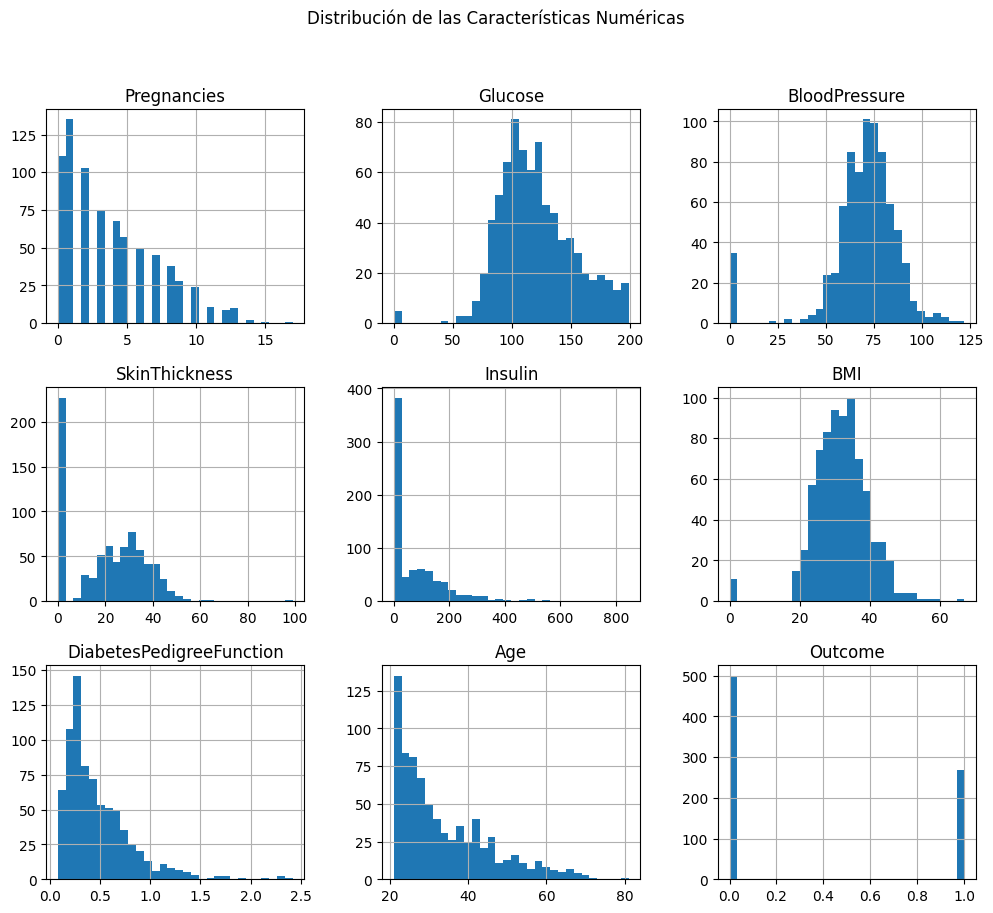
\includegraphics[width=\linewidth]{distribucion_caracteristicas.png}
\caption{Distribución de las Características Numéricas}
\label{fig:dist_caracteristicas}
\end{figure}

La Figura \ref{fig:dist_caracteristicas} nos proporciona información valiosa sobre la forma de las distribuciones de nuestras variables:

\begin{itemize}
    \item \textbf{Pregnancies}: Muestra una distribución asimétrica positiva (cola a la derecha), con la mayoría de los valores concentrados en el rango inferior.
    
    \item \textbf{Glucose}: Presenta una distribución aproximadamente normal, con un ligero sesgo hacia la derecha.
    
    \item \textbf{BloodPressure}: Exhibe una distribución casi simétrica, con una concentración de valores alrededor de 70-80 mm Hg.
    
    \item \textbf{SkinThickness}: Muestra una distribución multimodal, lo que podría indicar la presencia de subgrupos en la población o problemas en la medición de esta variable.
    
    \item \textbf{Insulin}: Presenta una distribución muy asimétrica positiva, con una gran cantidad de valores bajos y algunos valores extremadamente altos.
    
    \item \textbf{BMI}: Muestra una distribución ligeramente asimétrica positiva, con la mayoría de los valores entre 20 y 40.
    
    \item \textbf{DiabetesPedigreeFunction}: Exhibe una distribución muy asimétrica positiva, con la mayoría de los valores concentrados en el rango inferior y una cola larga hacia la derecha.
    
    \item \textbf{Age}: Presenta una distribución asimétrica positiva, con una mayor concentración de individuos jóvenes y adultos de mediana edad en la muestra.
\end{itemize}

\subsection{Análisis de Valores Únicos y Valores Atípicos}

Examinamos la cantidad de valores únicos en cada variable:

\begin{lstlisting}
Pregnancies                 17
Glucose                    136
BloodPressure               47
SkinThickness               51
Insulin                    186
BMI                        248
DiabetesPedigreeFunction   517
Age                         52
Outcome                      2
\end{lstlisting}

Destacamos que la variable objetivo 'Outcome' tiene 2 valores únicos, lo que confirma que estamos ante un problema de clasificación binaria.

Examinamos la presencia de valores atipicos mediante un boxplot:

\begin{figure}[h]
\centering
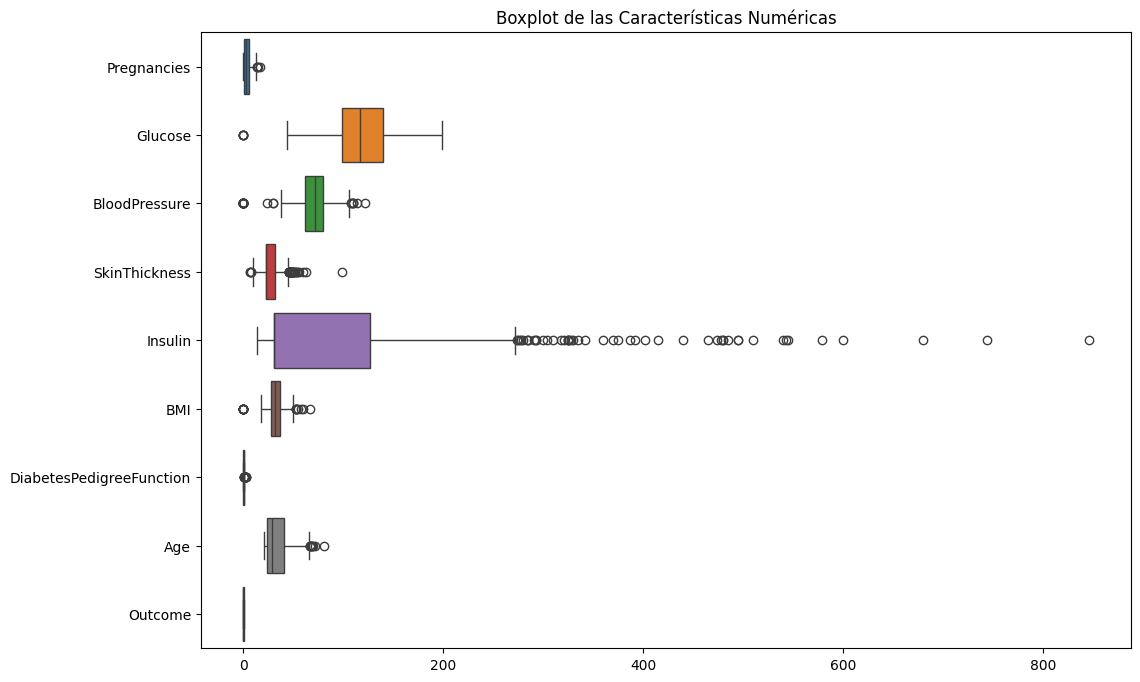
\includegraphics[width=\linewidth]{boxplot_caracteristicas.png}
\caption{Boxplot de las Características Numéricas}
\label{fig:boxplot}
\end{figure}

El boxplot (Figura \ref{fig:boxplot}) revela la presencia de valores atípicos en varias variables, especialmente en 'Insulin' y 'DiabetesPedigreeFunction'. Estos outliers podrían tener un impacto significativo en nuestros modelos y requerirán un análisis más detallado. 

Notamos gran cantidad de valores 0 en el boxplot (Figura \ref{fig:boxplot}) en ciertas características: 

\begin{lstlisting}
Glucose            5
BloodPressure     35
SkinThickness    227
Insulin          374
BMI               11
\end{lstlisting}

'SkinThickness' e 'Insulin' contienen muchos valores 0, lo cual es fisiológicamente improbable y comprometeria los resultados de nuestro modelo.

\subsection{Tratamiento de Valores Atípicos}

En este caso mantendremos los outliers encontrados en 'Insulin' y 'DiabetesPedigreeFunction' ya que creemos nos da valores autenticos y valiosos para el desarollo de nuestro modelo. En caso de afectar los resultados se usaria  IQR (Interquartile Range) para encontrar y reemplazar estos valores.

Para abordar el problema con los valores 0 en las características 'SkinThickness' e 'Insulin' , reemplazamos estos valores con la mediana de cada variable respectiva:

\begin{lstlisting}
df1['SkinThickness'] = df1['SkinThickness'].replace(0, df1['SkinThickness'].median())
df1['Insulin'] = df1['Insulin'].replace(0, df1['Insulin'].median())
\end{lstlisting}

Esta técnica de imputación nos permite conservar la distribución general de los datos mientras eliminamos valores potencialmente erróneos.

\subsection{Análisis de la Variable Objetivo}

Examinamos la distribución de la variable objetivo 'Outcome' para evaluar el balance de las clases:

\begin{figure}[h]
\centering
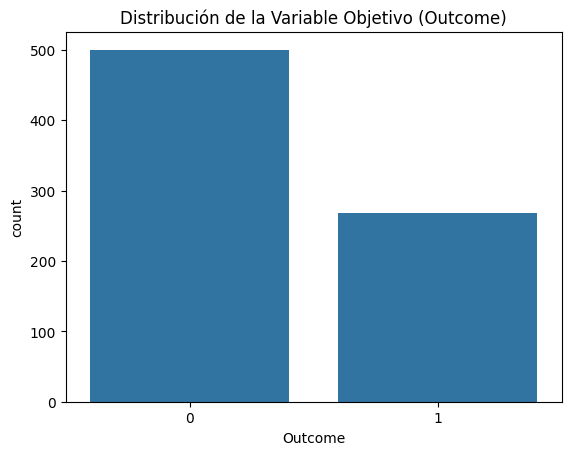
\includegraphics[width=\linewidth]{distribucion_outcome.png}
\caption{Distribución de la Variable Objetivo (Outcome)}
\label{fig:outcome_dist}
\end{figure}

La Figura \ref{fig:outcome_dist} muestra un desequilibrio en las clases, con una mayor proporción de casos negativos (sin diabetes) que positivos (con diabetes). Este desequilibrio deberá ser considerado durante la fase de modelado para evitar sesgos en nuestras predicciones.

\subsection{Análisis Bivariado}

Para comprender mejor la relación entre las variables predictoras y la variable objetivo, realizamos un análisis bivariado utilizando boxplots.

Para mostrar cómo se distribuyen las diferentes características en función del resultado (con o sin diabetes). Observamos diferencias notables en variables como 'Glucose', 'BMI' y 'Age' entre los dos grupos, lo que sugiere que estas variables podrían ser buenos predictores para nuestro modelo.

\section{Análisis Exploratorio de "Desgaste de Empleados"}

\section{Resultados de "Diabetes"}

\section{Resultados de "Desgaste de Empleados"}

\section{Discusión}

\section{Conclusiones}


\begin{thebibliography}{00}
\bibitem{b1} 
\end{thebibliography}



\end{document}
